
\documentclass[aps,twocolumn,secnumarabic,nobalancelastpage,amsmath,amssymb,
nofootinbib]{revtex4}

% nofootinbib is another document class option that allows you to put
% footnotes on the page where they occur rather than at the end of the
% paper.  This makes for easier reading!

% secnumarabic is a particularly nice way of identifying sections by
% number to aid electronic review and commentary.

% amsmath and amssymb are necessary for the subequations environment
% among others

\usepackage{chapterbib}
\usepackage{color}
\usepackage{graphics}      % standard graphics specifications
\usepackage{graphicx}      % alternative graphics specifications
\usepackage{longtable}     % helps with long table options
%\usepackage{url}          % for on-line citations (conflicts with hyperref)
\usepackage{bm}            % special 'bold-math' package
\usepackage[colorlinks=true]{hyperref}
\usepackage{listings}

\lstset{
  language=Python,
  showstringspaces=false,
  formfeed=\newpage,
  tabsize=4,
  commentstyle=\itshape,
  basicstyle=\ttfamily,
  morekeywords={models, lambda, forms}
}

\begin{document}
\title{The Cavendish Experiment}
\author         {Adnan Basar (Partner: Kadir Simsek)}
\email          {adnanbasarr@icloud.com}
\affiliation    {2010205108}
\date{\today}





\begin{abstract}
The object of this experiment is to measure the Gravitational Constant $G$.
\end{abstract}

\maketitle

%%%%%%%%%%%%%%%%%%%%%%%%%%%%%%%%%%%%%%%%%%%%%%%%%%%%%%%%%%%%%%%%%%
\section{Introduction}

Gravitation is one of few classes of interaction found in nature. Newton discovered in the 
${17}^{th}$ century that the same interaction that makes an apple fall from a tree is the same one 
that keeps the planets in orbit around the sun. Newton published the law of gravitation in 
1687, which states that: 
 \emph{\\
 \\
 Every particle of matter in the universe attracts every other particle with a 
force that is directly proportional to the product of the masses and inversely 
proportional to the square of the distance between them.\\}
\\

This is represented mathematically by:
\begin{center}

$F=\frac{G{m}_{1}{m}_{2}}{{r}^{2}}$

\end{center}
In the above equation $G$ refers to the universal gravitation constant which has units of ${kg}^{-1}{s}^{-2}$.However, more than a century elapsed before the magnitude of this constant was measured because the force is very small between any masses which could fit in a 
laboratory. It can be measured using a \emph{Torsion Balance}, which was used in 1798 by 
Cavendish to measure vale of $G$.\\


\begin{figure}[htbp]
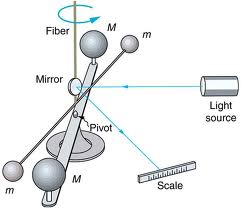
\includegraphics[width=2.5in]{setup.jpeg}
\caption{Experimental Setup}
\label{fig:schematic}
\end{figure}

Due to gravitational force between the one pair of small and large masses, there exists a net torque:

\begin{center}
$\tau=2Fd$
\end{center}

At the end this net torque and naturally opposing torque produced by the will result in a damped oscillation of the dumbbell. The equation of this oscillation is

\begin{center}
$I\frac{{d}^{2}\theta}{d{t}^{2}}+k\theta=0 $
\end{center}

where $I$ is the moment of inertia of the dumbbell system and k is the torsion constant of the wire used. Observing the oscillations through the displacement of a laser beam which is reflected off the small mirror spotted in the middle of the dumbbell and falls on a scale at a distance L, the universal gravitation constant can be determined as

\begin{center}
$G=\frac{{\pi}^{2}{b}^{2}dS}{M{T}^{2}{L}}$
\end{center}

where $b$ is the distance between the adjacent small and large massesi $M$ is the large mass, $2d$ is the length of the dumbbell, and S is the difference between the initial and the final equilibrium positions of the laser beam on the scale. $T$ is the period of the oscillation determined by requiring time for one successive wavelength.


\section{Experimental Setup}
Initial setted data for $M=1.498\ kg$, $d=0.050\ m$ and $b=0.0465\ m$

\begin{itemize}
\item Low Power Laser
\item Scale
\item Cavendish Torsion Balance With Large Masses
\item Ruler
\end{itemize}


\section{Data Analysis}
\begin{figure}[htbp]
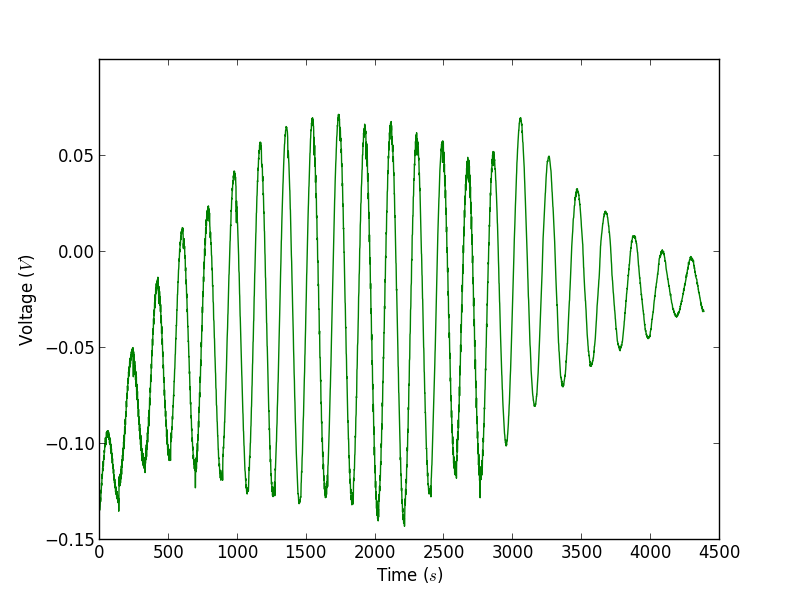
\includegraphics[width=2.5in]{figure_1}
\caption{Output of graph from Computer Cavendish Simulation Program}
\label{fig:schematic}
\end{figure}


Initially, we are some experiemtal data as in document \emph{cavendish RP2111.doc}
\begin{itemize}
\item $L=2\ m$
\item $\Delta{x}=0.03\ m$
\item $M=1.038\ kg$
\item $m=0.014\ kg$
\item $d=0.05\ m$
\item $R=0.05\ m$
\item $r= 0,0013\ m$
\item ${l}_{boom}=0,145\ m$ 
\item ${m}_{boom}=0.0071\ kg$
\item ${w}_{b}=0,0127\ m$
\item $b=0.46$
\end{itemize}

We are going to find $T$, the period of oscillation of the boom about the wire from Figure 2 as $252\ sec$.\\

In calculation parts,from the behaviours of the oscillation, we can calculate $k$ from
\begin{center}
$k=\left( \frac { 4{ \pi  }^{ 2 } }{ { T }^{ 2 } } +{ b }^{ 2 } \right) I$
\end{center}

where $I$ is the sum of the moments of inertia of the two small spheres ${ I }_{ s }=2\left( { m }{ d }^{ 2 }+\frac { 2 }{ 5 } m{ \frac{r}{2}}^{ 2 } \right) $ and the boom $ { I }_{ b }=\frac { m({ { l }_{ boom } }^{ 2 }+{ { w }_{ boom } }^{ 2 }) }{ 12 } $ where ${w}_{boom}$ is the width of the boom.\\

The displacement angle of a damped oscillator as a function of time is given by:
\begin{center}
$ \theta_{t}(t)=\theta_{e}+Ae^{-bt } cos(\omega{t}+\phi)$
\end{center}

By using derivations in References 3. we are going to have going to have corrected value $G$.\\

In corrected  form G is:

\begin{center}
$ G=\frac{k{\theta}_{D}{R}^{2}}{2Md((m-{m}_{h})(1-{f}_{d})+{m}_{b}{f}_{b})}$
\end{center}

\section{Results}
With the help of Python code, I did my calculation and I will  to Appendix part.\\

\begin{center}
\begin{table}[htbp]
\begin{tabular}{|l|c|c|r|}
\hline
{\small Results} & { \small Values } \\
\hline
${I}_{s}$& $0.000126$  \\
${I}_{b}$&  $1.25x10^{-5}$  \\
${I}$    &  $0.000138$  \\
${k}$    & $2.94x10^{-5}$   \\
${f}_{d}$& $0.035$   \\
${G}$& $7.86x10^{-11}$   \\



\hline
\end{tabular}

\end{table}
\end{center}



\section{Conclusions}
Error on G is : 
\begin{center}
$\frac{abs(6.67-7.86)}{6.67}=0.17 \rightarrow ~17\%$
\end{center}

The mass system is very sensitive and any little little perturbation may lead to make errors in our estimation. To make this smaller, we should use more isolated system. And initially we have setup in bad condition Fig. 2 shows that. Error may be better if we had better one. 


\section{References}
\begin{itemize}
\item E. Gulmez, ”Advanced Physics Experiment”, Istanbul, Bogazici University Publication, 1999
\item http://web.mit.edu/8.13/www/experiments.shtml
\item http://www.physics.uoguelph.ca/orbax/phys2440/GravitationalConstant.pdf
\end{itemize}

\section{Appendix}

Python for calculations:

\begin{lstlisting}

from pylab import *


m=0.0145
mb=0.0071
d=0.066
R=0.05
r=0.0013
lb=0.145
wb=0.0127
t=252.0
M=1038.0
b=0.046
td=0.19
mh=0.00034
fb=0.192


Is=2*(m*((d)**2)+2*m*((r/2.0)**2)/5.0)

print Is



inertia_b=mb*(lb**2+wb**2)/12.0
print inertia_b



I=Is+inertia_b
print I



k=(4*(pi)**2/((t)**2)+ b**2)*I
print k


fd=b**3/(b**2 + (2*d)**2)**(1.5)

print fd



G=k*td*(b)**2/2*M*d*((m-mh)*(1-fd)+mb*fb)
print G




\end{lstlisting}

\bibliography{photoelectric}


%%%%%%%%%%%%%%%%%%%%%%%%%%%%%%%%%%%%%%%%%%%%%%%%%%%%%%%%%%%%%%%%%%%%%%%%%%%%%
\begin{acknowledgments} 
I would like to thank my partner Kadir Simsek for his help to the experiment, and also to the teaching assistant Serhat Istin for his guidance during the experiment.

\end{acknowledgments}

%%%%%%%%%%%%%%%%%%%%%%%%%%%%%%%%%%%%%%%%%%%%%%%%%%%%%%%%%%%%%%%%%%%%%%%%%%%%%

\end{document}
